\subsection{アナログ入力そうち}\label{analog_in}
\subsubsection{感圧センサー}\label{touch}
\begin{table}[H]
	\begin{tabular}{|p{\colF}|p{\colG}|}	\hline
	名称 & 感圧センサー(かんあつせんさー)\\ \hline
	接続箇所 & アナログコネクタ (3pin)\\ \hline
	機能概要 & 圧力を測定する\\ \hline
  \end{tabular}
\end{table}

\begin{table}[H]
	\begin{tabular}{|p{\colF}|p{\colG}|}	\hline
	サンプルコードの場所 & ome/05/anain.hsp\\ \hline
	raspiへの入力 & 0~1023の値で圧力を測定します。圧力がかかるほど値が小さくなります。\\ \hline
	raspiへの入力方法 & val = spiget(ピン番号, チャンネル番号)\\ \hline
	raspiからの出力 & なし\\ \hline
	raspiからの出力方法 & なし\\ \hline
  \end{tabular}
\end{table}

\begin{table}[H]
	\begin{tabular}{|p{\colF}|p{\colG}|} \hline
	使い道 & 圧力を調べる、重さをはかる\\ \hline
	注意事項 & 圧力を感知する部分が壊れやすいです。\\ \hline
	補足 & なし\\ \hline
  \end{tabular}
\end{table}

\begin{figure}[H]
	\begin{tabular}{|p{\colH}|p{\colI}|p{\colH}|p{\colI}|} \hline
	外観 & 
	\begin{minipage}[t]{\linewidth}
    \smallskip
      \centering
      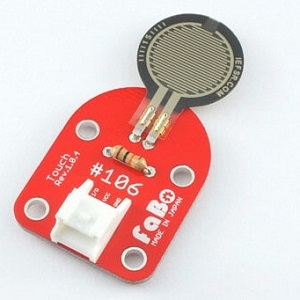
\includegraphics[width=\linewidth]{images/chap05/text05-img021.jpg}
      \caption{感圧センサー}
      \smallskip
    \end{minipage} &
    回路記号 & 
    \begin{minipage}[t]{\linewidth}
    \smallskip
      \centering
      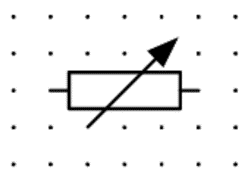
\includegraphics[width=\linewidth]{images/chap05/text05-img049.png}
      \caption{感圧センサーの回路図}
      \smallskip
    \end{minipage}\\ \hline
  \end{tabular}
\end{figure}